\documentclass[12pt]{article}
\usepackage[utf8]{inputenc}

\usepackage{enumitem}
\usepackage[margin=2cm]{geometry}

\usepackage{amsmath, amsfonts, amssymb}
\usepackage{graphicx}
\usepackage{tikz}
\usepackage{pgfplots}
\usepackage{multicol}

\usepackage{comment}
\usepackage{url}

\usepackage{titlesec}
\titleformat{\section}[frame]
{\normalfont\scshape}
{\thesection}{8pt}{\centering}

%\usepackage[margin=1cm]{cloze}

\usepackage[thmmarks]{ntheorem}

% MATH commands
\newcommand{\bC}{\mathbb{C}}
\newcommand{\bR}{\mathbb{R}}
\newcommand{\bN}{\mathbb{N}}
\newcommand{\bZ}{\mathbb{Z}}
\newcommand{\bT}{\mathbb{T}}
\newcommand{\bD}{\mathbb{D}}

\newcommand{\cL}{\mathcal{L}}
\newcommand{\cM}{\mathcal{M}}
\newcommand{\cP}{\mathcal{P}}
\newcommand{\cH}{\mathcal{H}}
\newcommand{\cB}{\mathcal{B}}
\newcommand{\cK}{\mathcal{K}}
\newcommand{\cJ}{\mathcal{J}}
\newcommand{\cU}{\mathcal{U}}
\newcommand{\cO}{\mathcal{O}}
\newcommand{\cA}{\mathcal{A}}
\newcommand{\cC}{\mathcal{C}}

\newcommand{\fK}{\mathfrak{K}}
\newcommand{\fM}{\mathfrak{M}}

\newcommand{\ga}{\left\langle}
\newcommand{\da}{\right\rangle}
\newcommand{\oa}{\left\lbrace}
\newcommand{\fa}{\right\rbrace}
\newcommand{\oc}{\left[}
\newcommand{\fc}{\right]}
\newcommand{\op}{\left(}
\newcommand{\fp}{\right)}

\newcommand{\ra}{\rightarrow}
\newcommand{\Ra}{\Rightarrow}

\renewcommand{\Re}{\mathrm{Re}\,}
\renewcommand{\Im}{\mathrm{Im}\,}
\newcommand{\Arg}{\mathrm{Arg}\,}
\newcommand{\Arctan}{\mathrm{Arctan}\,}
\newcommand{\sech}{\mathrm{sech}\,}
\newcommand{\csch}{\mathrm{csch}\,}
\newcommand{\Log}{\mathrm{Log}\,}
\newcommand{\cis}{\mathrm{cis}\,}

\newcommand{\ran}{\mathrm{ran}\,}
\newcommand{\bi}{\mathbf{i}}
\newcommand{\Sp}{\mathrm{span}\,}
\newcommand{\Inv}{\mathrm{Inv}\,}
\newcommand\smallO{
  \mathchoice
    {{\scriptstyle\mathcal{O}}}% \displaystyle
    {{\scriptstyle\mathcal{O}}}% \textstyle
    {{\scriptscriptstyle\mathcal{O}}}% \scriptstyle
    {\scalebox{.7}{$\scriptscriptstyle\mathcal{O}$}}%\scriptscriptstyle
  }
\newcommand{\HOL}{\mathrm{Hol}}
\newcommand{\cl}{\mathrm{clos}}
\newcommand{\ve}{\varepsilon}

\tikzstyle{myboxT} = [draw=black, fill=black!0,line width = 1pt,
    rectangle, rounded corners = 0pt, inner sep=8pt, inner ysep=8pt]
    
\newcommand{\MyC}[1]{\begin{tikzpicture}
\node (boxIntro) at (0,0) {};
\node [myboxT](Intro) at (boxIntro){%
	\begin{minipage}{0.9\textwidth}
	#1
	\end{minipage}};
\end{tikzpicture}}

%%%%  Environnement exer et solutionnaire
{\theorembodyfont{}
\theoremstyle{plain}
\theoremseparator{\textbf{.}}
\theoremsymbol{}
\newtheorem{exer}{\textbf{Exercise}}}

{\theorembodyfont{\color{blue}}
\theoremstyle{plain}
\theoremseparator{\textbf{:}}
\theoremsymbol{$\square$}
\newtheorem*{sol}{\textbf{Solution}}}

{\theorembodyfont{\color{blue}}
\theoremstyle{plain}
\theoremseparator{\textbf{:}}
\theoremsymbol{$\square$}
\newtheorem*{solWP}{\textbf{Solution}}}

{\theorembodyfont{\color{blue}}
\theoremstyle{plain}
\theoremseparator{\textbf{:}}
\theoremsymbol{$\square$}
\newtheorem*{hint}{\textbf{Hints}}}

\renewcommand*{\theexer}{\arabic{exer}}
\renewcommand*{\thesol}{\arabic{sol}}
\renewcommand*{\thesolWP}{\arabic{solWP}}
\renewcommand*{\thehint}{\arabic{hint}}

%%% Ignorer les solutions
\excludecomment{sol}
\excludecomment{solWP}
\excludecomment{hint}

\newcommand{\headHW}[4]{%
	\noindent \hrulefill \\
	MATH-#1 #2 \\
	#3 #4
	
}

\begin{document}
	\noindent \hrulefill \\
	MATH-331 Introduction to Real Analysis \hfill Pierre-Olivier Paris{\'e}\\
	Homework 01 \hfill Fall 2021\\\vspace*{-0.7cm}
	
	\noindent\hrulefill
	
	\noindent Due date: 09/06/2021 1:20pm \hfill Total: \hspace{0.3cm}/65.
	
\vspace*{1cm}

{\bf Instructions:} You must answer all the questions below and send your solution by email (to \url{parisepo@hawaii.edu}). If you decide to not use {\LaTeX} to hand out your solutions, please be sure that after you scan your copy, it is clear and readable. No late homework will be accepted. No format other than PDF will be accepted. Name your file as indicated in the syllabus.

\section{Homework problems}
\begin{exer}
(5 points) Prove that for any $n \in \bN$, $1 + 2 + \cdots + n = \frac{n(n + 1)}{2}$.
\end{exer}
\begin{sol}
We use induction on $n$. Let $P(n)$ be the proposition
	\begin{align*}
	\text{`` } 1 + 2 + \cdots + n = \frac{n (n + 1)}{2} \text{. "}
	\end{align*}
	\begin{itemize}
	\item For $n = 1$, we have $1 = 1\cdot 2/2$ and so $P(1)$ is true.
	\item Let $P(n)$ be true. Then, we have
		\begin{align*}
		\sum_{k = 1}^{n + 1} k = \sum_{k = 1}^n k + (n + 1)
		\end{align*}
	and from the induction hypothesis,
		\begin{align*}
		\sum_{k = 1}^{n + 1} k = \frac{n(n + 1)}{2} + (n + 1) = (n + 1) \Big( \frac{n}{2} + 1 \Big) = \frac{(n + 1)(n + 2)}{2}.
		\end{align*}
	So $P(n + 1)$ is true.
	\end{itemize}
By the PMI, $P(n)$ is true for any $n \in \bN$.
\end{sol}

\begin{exer}
(5 points)
Define $f : \bN \ra \bN$ by $f(1) = 1$, $f(2) = 2$ and $f(3) = 3$ and
	\begin{align*}
	f(n) := f(n - 1) + f(n- 2) + f(n -3) \quad (n \geq 4 ) .
	\end{align*}
Prove that $f(n) \leq 2^{n-1}$ for all $n \in \bN$.
\end{exer}
\begin{sol}
We will use second principle of mathematical induction on $n$. Let $P(n)$ be the proposition
	\begin{align*}
	\text{`` } f(n) \leq 2^{n-1} \text{. "}
	\end{align*}
	\begin{itemize}
	\item For $n = 1$, $n = 2$ and $n = 3$, $P(n)$ is true. Indeed, we have $f(1) = 1 \leq 1$, $f(2) = 2 \leq 2$ and $f(3) = 3 \leq 4$.
	\item Now take $n_0 = 3$ and suppose that $P(i)$ is true for any $1 \leq i \leq n$. We have
		\begin{align*}
		f(n + 1) = f(n) + f(n-1) + f(n -2 )
		\end{align*}	
	and using the induction hypothesis, we get
		\begin{align*}
		f(n + 1) \leq 2^{n-1} + 2^{n-2} + 2^{n-3} = 2^{n-3} (4 + 2 + 1) = 2^{n-3}\cdot 6 .
\end{align*}			
	Now, we know that $6 \leq 8$ (relative to the order $\leq$ on $\bN$) and so $f(n + 1) \leq 2^{n}$. This means that $P(n + 1)$ is true.	 
	\end{itemize}
By the PMI2, $P(n)$ is true for any $n \in \bN$.
\end{sol}

\begin{exer}
(5 points)
Prove that if $A$, $B$ and $C$ are sets, then
	\begin{enumerate}[label=\textbf{\alph*)}]
	\item $A \sim A$.
	\item If $A \sim B$, then $B \sim A$.
	\item If $A \sim B$ and $B \sim C$, then $A \sim C$.
	\end{enumerate}
\end{exer}
\begin{sol}
\begin{enumerate}
\item We can take $f(x) = 1_A (x) := x$, the identity function on the set $A$. This is a bijection.
\item Let $A \tilde B$. Then, by definition, there is a bijection $f : A \ra B$. Now, $f^-1: B \ra A$ exists (see your MATH 321 course) and is a bijection to. So, by definition, we get $B \tilde A$.
\item Suppose that $A \tilde B$ and $B \tilde C$. Then, by definition again, there are bijections $f : A \ra B$ and $g: B \ra C$. Define $h := g \circ f$ (the composition of $g$ with $f$). We have to show that $h$ is a bijection.
	\begin{itemize}
	\item \underline{Injectivity:} Let $h (x) = h(y)$. Then, $g(f(x)) = g(f(y))$. Since $g$ is injective, we infer that $f(x) = f(y)$ and using the injectivity of $f$, we get that $x = y$.
	\item \underline{Surjectivity:} Let $z \in C$. Since $g$ is surjective, there is a $y \in B$ such that $g(y) = z$. Also, $f$ is surjective. There is a $x \in A$ such that $f(x) = y$. Thus, we get $z = g(f(x)) = h(x)$.
	\end{itemize}
The function $h$ is the bijection that we were looking for. 
\end{enumerate}
\end{sol}

\begin{exer}
(5 points)
Show that any subset of a countable set is countable.
\end{exer}
\begin{sol}
Let $S$ be a countable set and let $E \subseteq S$. If $E$ is finite, then it is countable. Suppose that $E$ is infinite. Since $S$ is countable, there is a bijection $f: S \ra \bN$. Since $f$ is an injection, $f(E)$ is a subset of $\bN$ and must be infinite also. So, $f(E)$ is a non-empty infinite subset of $\bN$. By a Theorem of the lecture notes (Preliminaries-0), $f(E)$ is also countable. So there is a bijection $g : f(E) \ra \bN$. Now, the function $h : E \ra \bN$ defined by $h := g \circ f$ is the bijective function that we were looking for.
\end{sol}

%\begin{exer}
%Let $n \in \bN$ and $A_1$, $A_2$, $\ldots$, $A_n$ be countable sets. Show that $A_1 \times A_2 \times \cdots \times A_n$ is a countable set.
%\end{exer}
%\begin{sol}
%We will proceed by using the PMI on $n$. Let $P(n)$ be the proposition
%	\begin{align*}
%	\text{`` } A_1, A_2, \ldots, A_n \text{ countable sets } \Ra A_1 \times A_2 \times \cdots \times A_n \text{ is countable. "}
%	\end{align*}
	
%We know that $P(1)$ is true (by hypothesis) and we also know that $P(2)$ is true (see the lecture notes). Indeed, if $A_1$ is countable, then $A_1$ is countable. 

%Suppose that $P(n)$ is true. Let $A_1$, $A_2$, $\ldots$, $A_n$, $A_{n+1}$ be countable sets. By the induction hypothesis, since $A_1$, $A_2$, $\ldots$, $A_n$ are countable sets, we know that $A_1 \times A_2 \times \cdots \times A_n$ are also countable set. Then, since $P(2)$ is true, we can apply it to the sets $A_1 \times \cdots A_n$ and $A_{n + 1}$ to get that $A_1 \times \cdots \times A_n \times A_{n + 1}$ is a countable set. So, $P(n + 1)$ is true.

%By the PMI, $P(n)$ is true for any $n \in \bN$.
%\end{sol}



\begin{exer}
(10 points)
Let $0 < a < b$ be positive real numbers. Prove that
	\begin{enumerate}[label=\textbf{\alph*)}]
	\item $a^2 < b^2$.
	\item $\sqrt{a} < \sqrt{b}$.\label{Exo:squareInequality}
	\end{enumerate}
\end{exer}
\begin{sol}
\begin{enumerate}[label=\textbf{\alph*)}]
\item By the Axiom O4, we have that $a\cdot a < b \cdot a$. Similarly, by the Axiom O4, we have $a \cdot b < b \cdot b$. From the commutativity of the multiplication, we have $b a = ab$. By Axiom O2, we get that $a^2 < b^2$.
\item From Axiom O3, $\sqrt{a} < \sqrt{b}$, $\sqrt{a} = \sqrt{b}$, or $\sqrt{a} > \sqrt{b}$.
	\begin{itemize}
	\item Suppose that $\sqrt{a} = \sqrt{b}$. Then, by definition of the positive square-root, we have $(\sqrt{a})^2 = a$ and $(\sqrt{b})^2 = b$. So, $a = b$. This contradicts our hypothesis that $a < b$
	\item Suppose that $\sqrt{a} > \sqrt{b}$. Then, from a), we get $(\sqrt{b})^2 < (\sqrt{a})^2$ or equivalently, $b < a$. This last assumption contradicts our hypothesis saying that $a < b$.
	\end{itemize}
	So, we must conclude that $\sqrt{a} < \sqrt{b}$.
\end{enumerate}
\end{sol}

\begin{exer}
(5 points)
Sketch the region of the points $(x,y)$ satisfying the following relation: $x + |x| = y + |y|$ (explain your answer).
\end{exer}
\begin{sol}
There are four cases to consider:
	\begin{itemize}
	\item \underline{$x \geq 0$, $y \geq 0$}. In this case, we have $x + x = y + y$ and so $x = y$. Let $S_1:= \{ (x, y) \, : \, y = x \}$.
	\item \underline{$x \geq 0$, $y < 0$}. In this case, we have $x + x = y - y$ and so $x = 0$. Let $S_2 := \{ (0, y) \, : \, y < 0 \}$.
	\item \underline{$x < 0$, $y \geq 0$}. In this case, we have $x - x = y + y$ and so $y = 0$. Let $S_3:= \{ (x, 0) \, : \, x < 0 \}$.
	\item \underline{$x < 0$, $y < 0$}. In this case, we have $x - x = y - y$ and so the relation is always satisfied in this case. Let $S_4:=\{ (x, y) \, : \, x < 0, \, y < 0\}$.
	\end{itemize}

	\begin{figure}
	\centering
	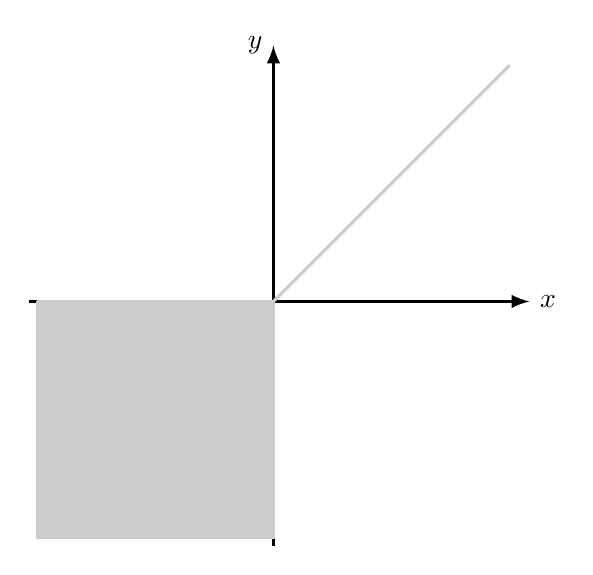
\begin{tikzpicture}
	\draw[black, very thick, ->, >=latex] (-3.1, 0) -- (3.25, 0)node[right]{$x$};
	\draw[black, very thick, ->, >=latex] (0, -3.1) -- (0, 3.25)node[left]{$y$};
	\draw[black!20, fill = black!20, very thick] (-3, 0) -- (0,0) -- (0, -3) -- (-3, -3) -- (-3, 0);
	\draw[black!20, very thick] (0,0) -- (3,3);
	\end{tikzpicture}
	\caption{Representation of the set $S_1 \cup S_2 \cup S_3 \cup S_4$}\label{fig:GraphOfRegion}
	\end{figure}
Figure \ref{fig:GraphOfRegion}, the region $\cup_{i = 1}^4 S_i$ is represented.
\end{sol}

\begin{exer}
(5 points)
If $x \geq 0$ and $y \geq 0$, prove that $\sqrt{xy} \leq \frac{x + y}{\sqrt{2}}$
\end{exer}
\begin{sol}
Let $x \geq 0$ and $y \geq 0$. Then, with a little algebra, we get $(x + y)^2 = x^2 + 2xy + y^2$. Now, since $x^2 \geq 0$ and $y^2 \geq 0$, we have 
	\begin{align*}
	(x + y)^2 = x^2 + 2xy + y^2 \geq 2xy \quad \Ra \quad xy \leq \frac{(x + y)^2}{2} .
	\end{align*}
Taking the square-root on each side and using exercise \ref{Exo:squareInequality}, we get $\sqrt{xy} \leq \frac{x + y}{\sqrt{2}}$.
\end{sol}

\begin{exer}
(10 points)
Find the infimum and supremum (if they exist) of the following sets. Make sure to justify all your answers:
	\begin{enumerate}[label=\textbf{\alph*)}]
	\item $E := \{ x \in \bR \, : \, x \geq 0 \text{ and } x^2 \leq 9 \}$.
	\item $E := \{ \frac{4n + 5}{n + 1} \, : \, n \in \bN \}$.
	\end{enumerate}
\end{exer}
\begin{sol}
\begin{enumerate}[label=\textbf{\alph*)}]
\item The set $E$ is bounded below by $0$ and $0 \in E$. So $\inf E = 0$. The set $E$ is also bounded above by $3$ because if $x > 3$, then $x^2 > 9$ and so $x \not\in E$. Since $3 \in E$, we have $\sup E = 3$.
\item We will find first the infimum and then the supremum.
	\begin{itemize}
	\item An upper bound for $E$ would be $\frac{9}{2}$. Indeed, we have $\frac{4n + 5}{n + 1} \leq \frac{9}{2}$ if and only if 
		\begin{align*}
		8n + 10 \leq 9n + 9 \iff 1 \leq n
		\end{align*}		 
	where the condition $n \geq 1$ is always satisfied. So, $\frac{4n + 5}{n + 1} \leq \frac{9}{2}$ for every $n \in \bN$. Also, $\frac{9}{2} \in E$ (just set $n= 1$) and so $\sup E = \frac{9}{2}$.
	\item A lower bound for $E$ would be $4$. Indeed, we have $\frac{4n + 5}{n + 1} > 4$ if and only if
		\begin{align*}
		4n + 5 > 4n + 4 \iff 1 > 0
		\end{align*}
	which is always true. So, $\frac{4n + 5}{n + 1} > 4$ for any $n \in \bN$ and this implies that $\inf E \geq 4$. We will show that $\inf E = 4$. Since $\inf E \leq 4$, we have $\inf E = 4$ or $\inf E > 4$. Let $x = \inf E$ and suppose that $x > 4$. By the Achimedian property with $x - 4 > 0$ in place of $x$ and $5 - x$ in place of $y$, there is a $n \in \bN$ such that
		\begin{align*}
		5 - x < n (x - 4)
		\end{align*}
	After some algebra, we get $\frac{4n + 5}{n + 1} < x$ which contradicts the definition of $x$ (it must be a lower bound for $E$). Then, we must take the other possibility, that is $\inf E = 4$.
	\end{itemize}
\end{enumerate}
\end{sol}

\section{Writing problems}
For each of the following problems, you will be ask to write a clear and detailed proof. You will have the chance to rewrite your solution in your semester project after receiving feedback from me.

\begin{exer}
(5 points)
Let $A$ be a non-empty set and $P(A)$ be its power set (the family of all subsets of $A$). Prove that $A$ is not equivalent to $P(A)$. Deduce that $P (\bN )$ is not countable. [Hint: Define $C := \{ x \,  :\, x \in A \text{ and } x \not\in f(x) \}$.]
\end{exer}
\begin{hint}
Argue by contradiction.	
	\begin{itemize}
	\item Suppose that $A \sim P (A)$. 
	\item Let $f : A \ra P (A)$ be a bijection between $A$ and $P(A)$ (why can you say that?).
	\item Define $C = \{ x \, : \, x \in A \text{ and } x \not\in f(x) \}$.
	\item There exists a $x \in A$ such that $f(x) = C$ (Why can you find such a $x$?).
	\item Can you answer the question "does $x \in f(x)$"? This should lead you to a contradiction.
	\end{itemize}
\end{hint}
\begin{solWP}
We want to show that there is no bijection between $A$ and $P(A)$. Suppose, on the contrary, that there is one. Let $f$ be this bijection. Let $C := \{ x \, : \, x \in A \text{ and } x \not\in f(x) \}$. Since $f$ is a bijection, there is a $x \in A$ such that $f(x) = C$. Now, we have two cases:
	\begin{itemize}
	\item If $C = \emptyset$. This implies that for any $x \in A$, $x \in f(x)$. But $f(x) = \emptyset$, so $x \in \emptyset$ and this implies that $A \subseteq \emptyset$. In other words, $A = \emptyset$. This is a contradiction with our assumption on $A$.
	\item If $C \neq \emptyset$. Do we have $x \in f(x)$? If $x \in f(x)$, then $x \not\in C$ (by definition of $C$). So, $x \in f(x) = C$ and $x \not\in C$, a contradiction! If $x \not\in f(x)$, then $x \in C$ (by definition of not being in $C$). So, $x \not\in f(x) = C$ and $x \in C$, a contradiction!
	\end{itemize}
So, the two cases lead to a contradiction and there is not such bijection between $A$ and $P(A)$.

Now, let $A = \bN$. Then, $\bN$ is not equivalent to $P (\bN )$. So, by definition of countability, $P (\bN )$ is not countable.
\end{solWP}

%\begin{exer}
%Let $p > 0$ and $n \in \bN$. Prove that there is a unique positive real number $x$ such that $x^n = p$.
%\end{exer}

\begin{exer}
(10 points)
Let $E \subseteq \bR$ be bounded from above and $E \neq \emptyset$. For $r \in \bR$, let
	\begin{align*}
	rE := \{ rx \, : \, x \in E \} \quad \text{ and } \quad r + E := \{ r + x \, : \, x \in E \} .
	\end{align*}
Show that
	\begin{enumerate}[label=\textbf{\alph*)}]
	\item if $r > 0$, then $\sup (r E) = r \sup (E)$.
	\item for any $r \in \bR$, $\sup (r + E) = r + \sup E$.
	\end{enumerate}
\end{exer}
\begin{hint}
First of all, $\sup E$ exists by the Axiom of completude (because $E$ is bounded from above). Set $s := \sup E$.

For a), you need to prove that
	\begin{itemize}
	\item $rx \leq rs$ for any $rx \in rE$, so that $rs$ is an upper bound for $rE$.
		\begin{itemize}
		\item For any $x \in E$, we know that $x \leq s$ (Why?).
		\item Which axiom can be used to get $rx \leq rs$. 
		\end{itemize}
	\item for any upper bound $b$ of $rE$, $rs \leq b$.
		\begin{itemize}
		\item Let $b$ be an upper bound for $rE$.
		\item Then, $rx \leq b$. Why can you conclude that $b/r$ is an upper bound for $E$?
		\item Then, $s \leq b/r$, Why should that be the case?
		\item Which axiom can be used to conclude.
		\end{itemize}
	\end{itemize}
	
For b), you follow the same guideline as before.
\end{hint}
\begin{solWP}
First of all, $\sup E$ exists by the Axiom of completude (because $E$ is bounded from above).
\begin{enumerate}[label=\textbf{\alph*)}]
\item Suppose that $r > 0$. Let $x \in E$ be arbitrary. Then, since $r > 0$ and $x \leq \sup E$, we have $rx \leq r \sup E$. Thus, $r \sup E$ is an upper bound for $rE$. By the Axiom of completude, $\sup (rE)$ exists and we also have $\sup (rE) \leq r \sup E$. 

We also have that $rx \leq \sup (rE)$ for any $x \in E$ and so, after a division by $r > 0$, we get $x \leq \sup (rE)/ r$ for any $x \in E$. Thus, $\sup (rE)/r$ is an upper bound for $E$ and we get that $\sup (E) \leq \sup (rE)/r$ which is equivalent to $r \sup (E) \leq \sup (rE)$. 

Combining this last inequality with the first one, we get $\sup (rE ) = r \sup (E)$.
\item Let $r \in \bR$. Let $x \in E$ be arbitrary. Then, since $x \leq \sup E$, we have $r + x \leq r + \sup (E)$. Thus, $r + \sup (E)$ is an upper bound for $r + E$. By the Axiom of completude, $\sup (r + E)$ exists and we get $\sup (r + E) \leq r + \sup (E)$.

However $r + x \leq \sup (r + E )$ for any $x \in E$. Thus, $x \leq \sup (r + E) - r$ and so $\sup (r + E) - r$ is an upper bound for $E$. Since $\sup (E)$ is the lower upper bound, we must have that $\sup (E) \leq \sup (r + E) - r$ and so $\sup (E) + r \leq \sup (r + E)$.

Combining this last inequality with the first one, we finally get that $\sup (r + E) = r + \sup (E)$.
\end{enumerate}
\end{solWP}

\end{document}

\begin{enumerate}[label=\textbf{\alph*)}]
\item Fix $n \geq 0$. Let $f : \cP_n \ra \bZ^{n + 1}$ be defined by
	\begin{align*}
	f( a_n x^n + a_{n - 1} x^{n- 1} + \cdots + a_1 x + a_0) = (a_n , a_{n - 1} , \ldots , a_1 , a_0 ) .
	\end{align*}
Then $f$ is injective. Indeed, if
	\begin{align*}
	f(a_n x^n + a_{n - 1} x^{n - 1} + \cdots + a_1 x + a_0 ) = f(b_n x^n + b_{n - 1} x^{n - 1} + \cdots + b_1 x + b_0 )
	\end{align*}
then $(a_n , a_{n - 1} , \ldots , a_0) = (b_n , b_{n - 1} , \ldots , b_0)$. This last equality implies that $a_i = b_i$ for every $0 \leq i \leq n$. So, by definition of equality between two polynomials, we get $a_n x^n + a_{n - 1} x^{n - 1} + \cdots + a_0 = b_n x^n + b_{n - 1} x^{n - 1} + \cdots + b_0$. 

We know that $\bZ$ is countable. By the last exercise, we also have that $\bZ^{n + 1}$ is countable. By a Corollary in the lecture notes, since $f$ is injective, the set $\cP_n$ must be countable also.
\item We can write $\cP = \cup_{n \geq 0} \cP_n$. Since each $\cP_n$ is countable (from a)), by a Theorem in the lecture notes, we deduce that $\cP$ (as the union of all $\cP_n$) is also countable.
\end{enumerate}